\chapter{Resultados}


\section{Estudio sobre la influencia de marcadores en el declive cognitivo en la Enfermedad del Parkinson}

Como resultado de la realización del algoritmo anterior, se obtuvieron las dos tablas siguientes, con las que se realizará un estudió de las variables:

\begin{description}
	\item{\textbf{Tabla 1:}} comparativa entre pacientes PD y el grupo de control en la linea de base.
	
	En la tabla \ref{tab:tabla1}, se observa como para cada grupo se muestra, en el caso de las variables cualitativas, el valor medio de sujetos y mujeres y su porcentaje en comparación con el total; y en el caso de las características cuantitativa, la media, la desviación típica y los máximos y mínimos. Además, se marca con una \textit{a} en la columna 'post-hoc' cuales de ellas son indicativas del declive cognitivo al inicio del estudio.
	
	
	\begin{table}[t]
		\begin{adjustbox}{width=\textwidth}
			\begin{tabular}{|l||c|c|c|}
				\toprule
				Group &                                 PD &                                 HC & Post-hoc \\
				\midrule
				Subjects &                        423 (61.9\%) &                        196 (28.7\%) &    -      \\
				Female &                        146 (34.5\%) &                         70 (35.7\%) &  -    \\
				APOE4 &                  101 (26.3\%) n=384 &                   47 (26.4\%) n=178 &   -   \\
				Age &            61.7 (9.7) (33.5, 84.9) &           60.8 (11.2) (30.6, 83.7) &  -    \\
				Education &         15.56 (2.97) (5.00, 26.00) &         16.04 (2.89) (8.00, 24.00) &   -   \\
				\hline
				GDS &          2.32 (2.44) (0.00, 14.00) &          1.29 (2.10) (0.00, 15.00) &        a \\
				UPSIT &         22.35 (8.23) (1.00, 40.00) &        33.98 (4.86) (11.00, 40.00) &        a \\
				REM &          4.12 (2.69) (0.00, 12.00) &          2.83 (2.26) (0.00, 11.00) &        a \\
				UPDRS3 &         20.89 (8.85) (4.00, 51.00) &          1.21 (2.19) (0.00, 13.00) &        a \\
				\hline
				\multicolumn{4}{ |l| }{Cognitive outcomes} \\
				\hline
				MOCA &        27.13 (2.32) (17.00, 30.00) &        28.23 (1.11) (26.00, 30.00) &        a \\
				LNS &         10.59 (2.66) (2.00, 20.00) &         10.87 (2.57) (2.00, 20.00) &   -   \\
				SDMT &         41.18 (9.73) (7.00, 82.00) &       46.77 (10.53) (20.00, 83.00) &        a \\
				JLO &         12.77 (2.13) (5.00, 15.00) &         13.12 (1.98) (4.00, 15.00) &  -    \\
				INMEDIATE &         24.44 (4.98) (9.00, 36.00) &        26.05 (4.50) (15.00, 35.00) &        a \\
				HVLTRDLY &          8.36 (2.52) (0.00, 12.00) &          9.29 (2.32) (2.00, 12.00) &        a \\
				SFT &      48.67 (11.63) (20.00, 103.00) &       51.80 (11.20) (22.00, 80.00) &        a \\
				ADL &       93.14 (5.89) (70.00, 100.00) &      100.00 (0.00) (100.00, 100.00) &  -    \\
				SCOPA &          9.51 (6.18) (0.00, 39.00) &          5.83 (3.69) (0.00, 20.00) &        a \\
				\hline
				\multicolumn{4}{ |l| }{CSF and DAT imaging markers} \\
				\hline
				ABETA &  909.55 (410.73) (238.80, 3707.00) & 1019.37 (499.46) (239.10, 3297.00) &        a \\
				ASYN & 1506.70 (666.59) (432.40, 5256.90) & 1695.19 (747.42) (488.60, 4683.10) &        a \\
				TAU &     169.54 (56.80) (80.93, 467.00) &     191.64 (79.26) (81.96, 580.80) &        a \\
				PTAU &         14.87 (5.25) (8.01, 40.13) &         17.52 (8.35) (8.08, 73.61) &        a \\
				pTauAB &           0.02 (0.01) (0.01, 0.08) &           0.02 (0.02) (0.01, 0.18) &  -    \\
				MEANPUT &           0.83 (0.30) (0.24, 2.17) &           2.15 (0.56) (0.64, 3.89) &        a \\
				MEANCAU &           2.00 (0.56) (0.39, 3.71) &           2.98 (0.63) (1.32, 5.20) &        a \\
				\bottomrule
			\end{tabular}
		\end{adjustbox}
		\caption{Características clínicas y demográficas}
		\label{tab:tabla1}
	\end{table}
	
	
	
	
	\item{\textbf{Tabla 2:}} comparativa entre la evolución de los pacientes con Parkinson a los distintos grupos (PD\_CU, PD\_MCI y PDD).
	
	En la tabla \ref{tab:tabla2}, se realizan los mismos cálculos estadísticos de la tabla \ref{tab:tabla1}, ya que permiten visualizar la influencia de los distintos parámetros en la evolución de los tres grupos expuestos. Con las columnas 'p-value' y 'post-hoc' se reflejan las variables que son significativas para predecir el avance de la enfermedad a cada uno de los grupos y que permitirían pronosticar si el paciente puede desarrollar deterioro cognitivo medio o demencia en las primeras fases de la enfermedad.
	
	\begin{table}[t]
		\begin{adjustbox}{width=\textwidth}
			\begin{tabular}{|l||c|c|c|c|c|}
				\toprule
				Group &                              PD\_CU &                             PD\_MCI &                        PDD &   p-value & Post-hoc \\ 
				\midrule
				Subjects &                        323 (47.3\%) &                         83 (12.2\%) &                          17 (2.5\%) &     -      &    -      \\
				Female &                        120 (37.2\%) &                         20 (24.1\%) &                          6 (35.3\%) &     0.083 &  -    \\
				APOE4 &                   78 (26.4\%) n=295 &                    18 (23.7\%) n=76 &                     5 (38.5\%) n=13 &     0.101 &  -    \\
				Age &            60.1 (9.8) (33.5, 82.3) &            66.0 (7.4) (48.0, 84.9) &            69.4 (7.4) (54.8, 83.0) & $<$ 0.001 &      a,b \\
				Education &         15.70 (2.87) (8.00, 26.00) &         14.99 (2.82) (8.00, 21.00) &         15.59 (4.91) (5.00, 21.00) &     0.150 &  -    \\
				\hline
				GDS &          2.17 (2.40) (0.00, 14.00) &          2.86 (2.61) (0.00, 13.00) &           2.71 (2.11) (0.00, 8.00) &     0.058 &   -   \\
				UPSIT &         23.41 (7.87) (5.00, 39.00) &         19.54 (8.60) (1.00, 40.00) &         16.06 (7.39) (5.00, 31.00) & $<$ 0.001 &      a,b \\
				REM &          3.82 (2.54) (0.00, 12.00) &          5.06 (2.90) (0.00, 12.00) &          5.24 (3.11) (0.00, 12.00) & $<$ 0.001 &        a \\
				UPDRS3 &         20.51 (8.73) (5.00, 47.00) &         22.29 (9.40) (4.00, 51.00) &        21.29 (8.18) (10.00, 39.00) &     0.260 &  -    \\
				\hline
				\multicolumn{6}{|l|}{Cognitive outcomes} \\
				\hline
				MOCA &        27.33 (2.17) (19.00, 30.00) &        26.58 (2.70) (17.00, 30.00) &        25.94 (2.38) (21.00, 29.00) &     0.003 &    -      \\
				LNS &         11.04 (2.50) (2.00, 20.00) &          9.29 (2.58) (4.00, 17.00) &          8.29 (2.78) (3.00, 13.00) & $<$ 0.001 &      a,b \\
				SDMT &        42.94 (8.75) (17.00, 82.00) &        36.69 (10.18) (7.00, 58.00) &       29.82 (10.85) (15.00, 50.00) & $<$ 0.001 &      a,b \\
				JLO &         12.98 (1.96) (5.00, 15.00) &         12.19 (2.44) (6.00, 15.00) &         11.53 (2.67) (6.00, 15.00) & $<$ 0.001 &        a \\
				INMEDIATE &         25.26 (4.74) (9.00, 36.00) &        22.13 (4.90) (11.00, 34.00) &        20.24 (4.28) (14.00, 28.00) & $<$ 0.001 &      a,b \\
				HVLTRDLY &          8.75 (2.35) (0.00, 12.00) &          7.13 (2.75) (0.00, 12.00) &          7.00 (2.12) (3.00, 11.00) & $<$ 0.001 &        a \\
				SFT &      50.60 (11.54) (24.00, 103.00) &        43.48 (9.39) (20.00, 70.00) &        37.35 (9.37) (25.00, 54.00) & $<$ 0.001 &      a,b \\
				ADL &       93.25 (6.02) (70.00, 100.00) &       93.01 (5.29) (80.00, 100.00) &       91.76 (6.11) (80.00, 100.00) &     0.583 &   -   \\
				SCOPA &          8.74 (5.70) (0.00, 35.00) &         11.79 (6.96) (3.00, 39.00) &         13.06 (7.20) (4.00, 32.00) & $<$ 0.001 &        a \\
				\hline
				\multicolumn{6}{|l|}{CSF and DAT imaging markers} \\
				\hline
				ABETA &  942.40 (413.12) (315.90, 3707.00) &  844.08 (395.26) (238.80, 2572.00) &  592.27 (251.10) (308.80, 1300.00) &     0.001 &        b \\
				ASYN & 1519.17 (680.58) (432.40, 5256.90) & 1470.97 (620.62) (472.00, 3443.70) & 1443.49 (642.42) (539.40, 2780.50) &     0.783 &  -    \\
				TAU &     167.17 (54.61) (80.93, 467.00) &     172.53 (59.27) (83.93, 345.30) &     202.68 (78.07) (97.17, 327.40) &     0.053 &   -   \\
				PTAU &         14.52 (4.99) (8.02, 40.13) &         15.51 (5.40) (8.36, 32.80) &         18.59 (7.68) (8.01, 30.84) &     0.007 &        b \\
				pTauAB &   0.0161 (0.0071) (0.0063, 0.0673) &   0.0196 (0.0120) (0.0103, 0.0816) &   0.0337 (0.0169) (0.0138, 0.0698) & $<$ 0.001 &      b,c \\
				MEANPUT &           0.85 (0.29) (0.24, 2.15) &           0.77 (0.32) (0.29, 2.17) &           0.66 (0.18) (0.31, 1.05) &     0.005 &    -      \\
				MEANCAU &           2.07 (0.54) (0.39, 3.71) &           1.80 (0.54) (0.62, 3.27) &           1.59 (0.50) (0.74, 2.52) & $<$ 0.001 &      a,b \\ 
				\bottomrule
			\end{tabular}
		\end{adjustbox}
		\caption{Características clínicas y demográficas}
		\label{tab:tabla2}
	\end{table}
	
\end{description}






\section{Análisis longitudinal y reconstrucción temporal de un único sujeto}
Como resultado del algoritmo desarrollado para el análisis temporal del individuo, se obtienen varias gráficas. Se representa tanto la convergencia de algunos parámetros estimados, como las curvas de la variables para el individuo indicado.\\

\subsection{Convergencia de los parámetros grupales}
Tras ejecutar \textbf{leaspy.fit}, el programa realiza las 50 iteraciones indicadas para conseguir calcular los parámetros grupales que mejor se aproximen a la trayectoria real del conjunto. También hay que tener en cuenta que un algoritmo tiene que ser optimo y eficaz, pero con una velocidad de ejecución no muy alta, ya que podría llegar a ser un inconveniente. Por lo que se consideró que 50 iteraciones era una cifra óptima para lograr el objetivo deseado. \\

EL algoritmo guarda los valores de los factores grupales de cada ciclo y con formato CSV en el directorio :
\begin{center}
	\texttt{Demos/rroca\_python/pred\_sujeto/logs/parameter\_convergence} 
\end{center}

Al mismo tiempo, utiliza los datos registrados para generar una gráfica para cada uno de los biomarcadores para comprobar la correcta convergencia de los mismo. Cada una representa uno de los parámetros del \textit{'long-term'}: \textit{g, v0, source, tau y xi}. Los tres últimos constan de dos gráficas, ya que se refleja tanto la media de dichos indicadores como la desviación estandar.\\

\begin{figure}[h]
	\centering
	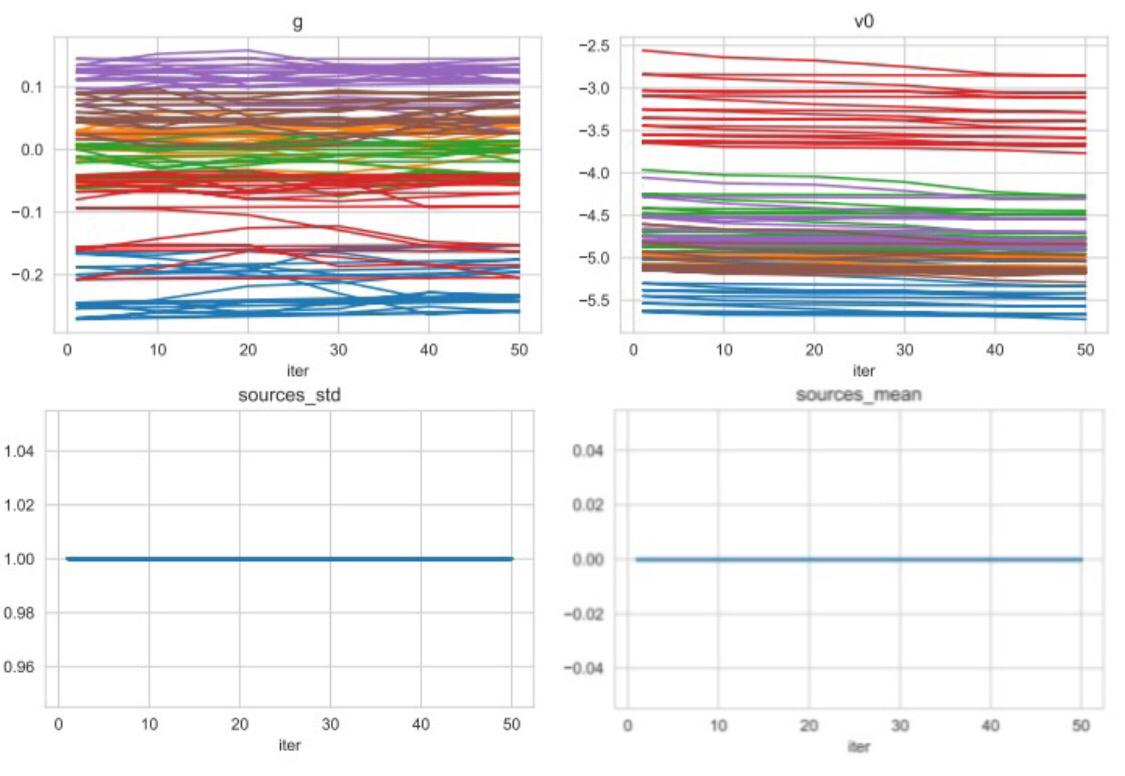
\includegraphics[width=1\textwidth]{imagenes/conv1_gvsource.jpg}
	\caption{Convergencia de g, v0 y source.}
	\label{fig:conv1_gvsource}
\end{figure}
\begin{figure}[h]
	\centering
	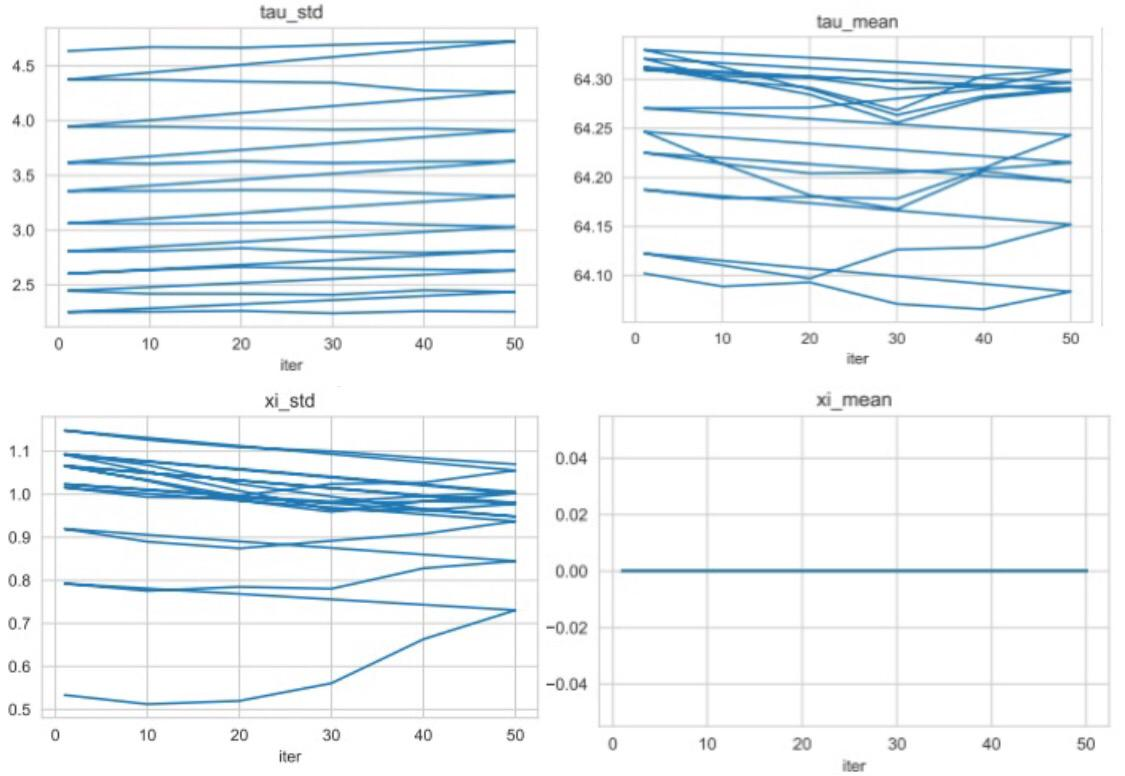
\includegraphics[width=1\textwidth]{imagenes/conv1_tauxi.jpg}
	\caption{Convergencia de tau y xi.}
	\label{fig:conv1_tauxi}
\end{figure}
\begin{figure}[h]
	\centering
	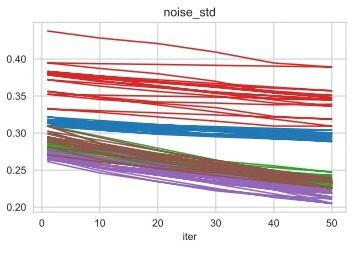
\includegraphics[width=0.7\textwidth]{imagenes/conv1_noise.jpg}
	\caption{Convergencia de noise.}
	\label{fig:conv1_noise}
\end{figure}


En el eje 'x' de cada cuadro se puede el número de iteración al que corresponde cada medida aproximada, mientras que en el eje 'y' se observa el valor del parámetro correspondiente. Los valores correspondientes a variable medida del paciente se gráfica con un color distinto en el caso de \textit{g}, \textit{v0} y \textit{noise}.Hay seis colores diferentes en cada una de estas gráfica, ya que se ha hecho el estudio para seis marcadores distintos: ABETA, HVLTRDLY, LNS, MEANCAU, SDMT y SFT. Por otra parte, cada linea representa las estimaciones de cada uno de los 10 modelos generados.\\

\subsection{Curvas características individuales}
Por otro lado, se gráfican las trayectorias \textit{'short-term'} que representan la estimación de la progresión de cada uno de los marcadores del paciente escogido.\\

El programa genera dos conjunto de seis cuadros para cada uno de los 10 modelos, siendo cada cuadro la estimación de los valores de una variable y el primer conjunto grafica los números normalizados de las mismas y el segundo en escala original. Es decir, se obtienen un total de veinte conjuntos con seis gráficas en su interior, ya que se trabaja con un bootstrap de valor 10, lo que indica que se generan 10 modelos. \\

Además de representarse en cada cuadro la curva estimada, se indican los valores de cada variable en cada observación del paciente con un punto, para así poder ver cuan precisa es la estimación de la trayectoria a corto plazo.\\

De manera ilustrativa, en este documento se muestran las gráficas dibujadas para el modelo número cinco,  viendo en primer lugar los valores normalizados para las seis variables escogidas en la imagen\ref{fig:trayM5norm} y después las curvas para los valores originales en la figura \ref{fig:trayM5orig}.\\

\begin{figure}[h]
	\centering
	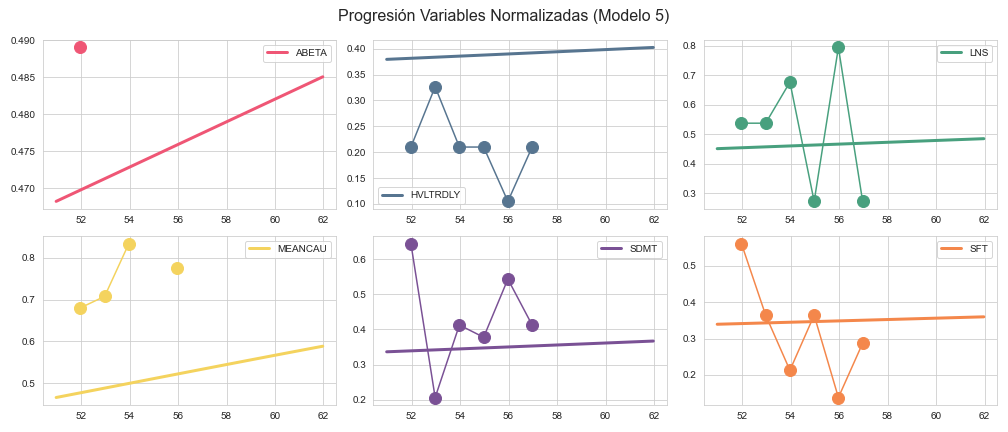
\includegraphics[width=1\textwidth]{imagenes/trajectory_norm_plot_model_5.png}
	\caption{Trayectoria Normalizada del modelo 5.}
	\label{fig:trayM5norm}
\end{figure}

\begin{figure}[h]
	\centering
	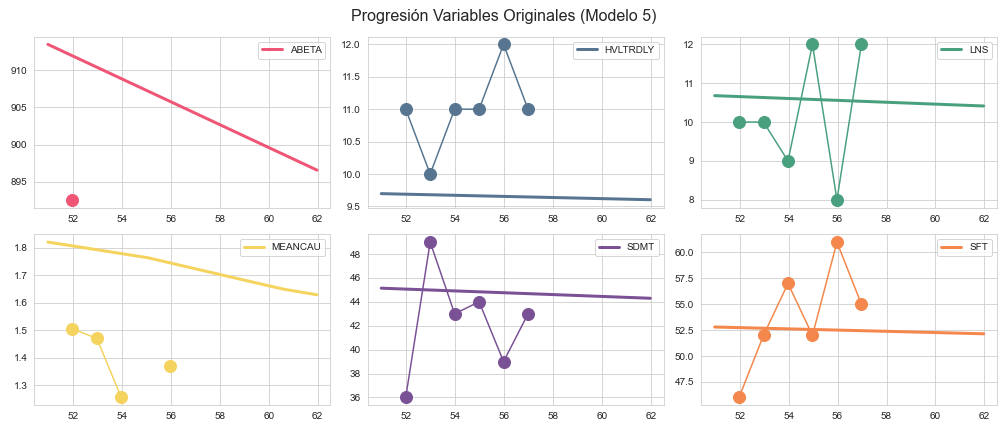
\includegraphics[width=1\textwidth]{imagenes/trajectory_orig_plot_model_5.png}
	\caption{Trayectoria original del modelo 5.}
	\label{fig:trayM5orig}
\end{figure}

El resto de representaciones se pueden encontrar en la siguiente ruta del proyecto:
\begin{center}
		\texttt{Demos/rroca\_python/pred\_sujeto/\\
		plots/norm\_orig}. 
\end{center}


\section{Modelos de progresión con múltiples sujetos}
Como resultados se obtienen los parámetros correspondientes a las prestaciones de los DPMs. Con ellos se podrán comparar las predicciones tanto de la progresión de la enfermedad en los distintos pacientes, como el pronóstico estimado y el estado cognitivo de los mismos. \cite{ghazi2021robust} Las distintas prestaciones se clasifican en función de lo que miden:\\





\subsection{Evaluación de las trayectorias estimadas}
Para comprobar la rigurosidad de las trayectorias \textit{short-term} estimadas, se implementa la estimación del NMAE. Para cada modelo, es la media de la diferencias entre las estimaciones en escala normalizada y las muestras en cada tiempo muestreado. Cada una de las variables obtiene valor de un NMAE.\\

Además, se consiguió realizar la interpolación inversa de los valores para obtener el error medio absoluto (MAE) en la escala original de cada biomarcador. Se calculó la media para el conjunto de pacientes tanto de entrenamiento como de test para cada uno de los bootstraps y para cada una de las variables de cada modelo estimado. \\

Las distintas tablas para estas prestaciones se guardan en los directorios creados para cada uno de los modelos en la siguiente carpeta: 

\begin{center}
	\texttt{Demos/rroca\_python/multi\_leaspy/outputs/prestaciones} 
\end{center}

Por ejemplo, en la tabla \ref{tab:mae train} se encuentran los valores del MAE para el modelo estimado formado por las variables moca, gds, rem y lns para los pacientes de entrenamiento y en la tabla \ref{tab:mae test} para los pacientes de test.

\begin{table}[htbp]
	\centering
	\begin{tabular}{|c|c|c|c|c|}
		\hline
		-& moca & gds & rem & lns \\
		\hline
		0 & 1.875753365 & 1.883087673 & 2.381450853 & 1.701934104 \\
		1 & 1.857000425 & 1.926429807 & 2.173352265 & 1.748594863 \\
		2 & 1.810034038 & 1.809383412 & 2.146301583 & 1.782876384 \\
		3 & 1.82706661 & 1.904189807 & 2.142610773 & 1.843265758 \\
		4 & 1.809876103 & 1.922792541 & 2.069831685 & 1.783131133 \\
		5 & 1.859018366 & 1.957659282 & 1.989934764 & 1.800958343 \\
		6 & 1.827878927 & 2.009812252 & 2.062568052 & 1.767653103 \\
		7 & 1.790537378 & 2.00620193 & 2.075641576 & 1.771343093 \\
		8 & 1.784458749 & 1.957341924 & 2.116083299 & 1.747069773 \\
		9 & 1.787830739 & 2.013548435 & 2.193212644 & 1.739714307 \\
		\hline
	\end{tabular}
	\caption{MAE para los pacientes de entrenamiento del modelo formado por las variables moca, gds, rem y lns con índices 1, 2, 4 y 7}
	\label{tab:mae train}
\end{table}

\begin{table}[htbp]
	\centering
	\begin{tabular}{|c|c|c|c|c|}
		\hline
		- & moca & gds & rem & lns \\
		\hline
		0 & 1.99110532 & 1.818498919 & 2.309924046 & 1.686225067 \\
		1 & 1.960751042 & 1.875013754 & 2.124774943 & 1.714485756 \\
		2 & 1.885138411 & 1.751960495 & 2.084473015 & 1.734213722 \\
		3 & 1.916702223 & 1.882623832 & 2.095779037 & 1.782219241 \\
		4 & 1.891402283 & 1.879699705 & 2.006357296 & 1.733370327 \\
		5 & 1.960049566 & 1.925798991 & 1.94639827 & 1.743088832 \\
		6 & 1.912919106 & 1.972329063 & 2.011377444 & 1.721898135 \\
		7 & 1.879662528 & 1.969527728 & 2.014229037 & 1.737797063 \\
		8 & 1.884606227 & 1.912281928 & 2.052043181 & 1.719957491 \\
		9 & 1.881427765 & 1.983761287 & 2.12839662 & 1.715905914 \\
		\hline
	\end{tabular}
	\caption{MAE para los pacientes de prueba del modelo formado por las variables moca, gds, rem y lns con índices 1, 2, 4 y 7}
	\label{tab:mae test}
\end{table}

En el caso de los valores normalizados de este parámetro (NMAE) se realizó el mismo proceso obteniendo las mismas tablas (\ref{tab:NMAE train},\ref{tab:NMAE test}) para los dos grupos de pacientes indicados: 

\begin{table}[htbp]
	\centering
	\begin{tabular}{|c|c|c|c|c|}
		\hline
		-& MOCA\_n & GDS\_n & REM\_n & JLO\_n \\
		\hline
		0 & 0.175080174 & 0.250673513 & 0.244964451 & 0.19293362 \\
		1 & 0.174266868 & 0.258983794 & 0.232132703 & 0.199171354 \\
		2 & 0.174922013 & 0.260575615 & 0.217134551 & 0.197051628 \\
		3 & 0.176274691 & 0.265997893 & 0.223300401 & 0.201590661 \\
		4 & 0.179186227 & 0.260825316 & 0.24498487 & 0.202679124 \\
		5 & 0.179737067 & 0.261089166 & 0.235326641 & 0.203301559 \\
		6 & 0.173299094 & 0.263228934 & 0.224328989 & 0.198079031 \\
		7 & 0.180172049 & 0.264731444 & 0.232004545 & 0.201174008 \\
		8 & 0.179942543 & 0.264649857 & 0.223606286 & 0.200609576 \\
		9 & 0.18113462 & 0.265606441 & 0.233126432 & 0.200776704 \\
		\hline
	\end{tabular}
	\caption{NMAE para los pacientes de entrenamiento del modelo formado por las variables moca, gds, rem y lns con índices 1, 2, 4 y 7}
	\label{tab:NMAE train}
\end{table}

\begin{table}[htbp]
	\centering
	\begin{tabular}{|c|c|c|c|c|}
		\hline
		-& MOCA\_n & GDS\_n & REM\_n & JLO\_n \\
		\hline
		0 & 0.169347919 & 0.246232739 & 0.239188087 & 0.19168615 \\
		1 & 0.169065739 & 0.254223242 & 0.226459231 & 0.198219059 \\
		2 & 0.17078571 & 0.255086216 & 0.210715076 & 0.19600423 \\
		3 & 0.171183584 & 0.262244499 & 0.21821739 & 0.200535896 \\
		4 & 0.172741525 & 0.257764461 & 0.237596966 & 0.201031517 \\
		5 & 0.172639815 & 0.258459964 & 0.228133037 & 0.201466419 \\
		6 & 0.16603492 & 0.262330962 & 0.218097098 & 0.196039254 \\
		7 & 0.173392834 & 0.262801125 & 0.225295884 & 0.199740264 \\
		8 & 0.173107566 & 0.262273215 & 0.217208888 & 0.198831721 \\
		9 & 0.174414623 & 0.263279289 & 0.226875962 & 0.198469437 \\
		\hline
	\end{tabular}
	\caption{NMAE para los pacientes de test del modelo formado por las variables moca, gds, rem y lns con índices 1, 2, 4 y 7}
	\label{tab:NMAE test}
\end{table}

\subsection{Clasificación del estado clínico}
Para clasificar el estado cognitivo se utiliza  un clasificador bayesiano basado en el 'Disease Progresion Score'(DPS)($s_{ij}$) y que utiliza un kernel de estimación de la densidad (KDE) basado en estimaciones acordes.
\begin{center}
	$s_{ij}=\alpha_{i}t_{ij}+\beta_{i}$
\end{center}

La estimación de esta prestación todavía se haya en desarrollo, por lo que no es posible facilitar sus resultados por el momento. 

\subsection{Medidas relacionadas con los plazos de conversión hacia el declive cognitivo}
Para la medida de estas prestaciones se utilizan cuatro parámetros: SCORE1, SCORE2, SCORE3, SCORE4. Con ellos se calcula la precisión de los modelos para estimar el estado del declive cognitivo en el que se encuentran los pacientes. Con leaspy se estima el tiempo de conversión al declive cognitivo de los distintos individuos. En función de si la edad de conversion es menor o mayor que la primera y última observación, se sabe si el paciente corresponde al grupo de los SCU, los cuales convierten después de la última observación, a los sMCI si convierte antes de la primera visita, o a los pCU si convierte entre la primera y la ultima visita. Los valores obtenidos de los SCORES se muestran en la imagen \ref{fig:SCORES}\\
\begin{itemize}
	\item El SCORE1 mide el porcentaje de pacientes sCU que ha estimado el algoritmo en proporción a los sCU reales. 
	\item El SCORE2 calcula el porcentaje de pacientes sMCI en proporción de los sMCI reales.
	\item El SCORE3 y el SCORE4 calculan el porcentaje de pacientes pCU en comparación con los pCU reales.
\end{itemize}
\begin{figure}[h]
	\centering
	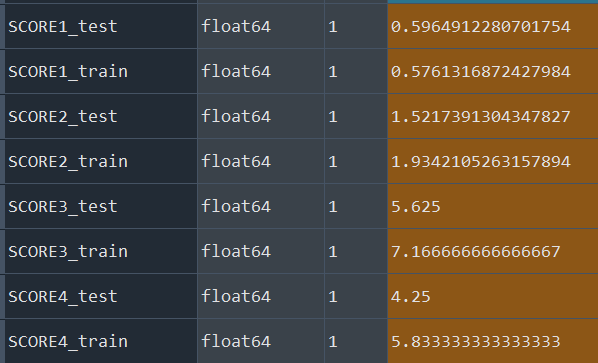
\includegraphics[width=0.5\textwidth]{imagenes/SCORES1,2,3,4.PNG}
	\caption{SCORES estimados}
	\label{fig:SCORES}
\end{figure}



